\documentclass[11pt,a4paper]{article}
\usepackage[margin=27mm]{geometry}
\usepackage{fontspec,unicode-math,amsmath,booktabs,graphicx,hyperref}
\setmainfont{STIXGeneral}\setmathfont{STIX Two Math}
\setlength{\parindent}{0pt}\setlength{\parskip}{6pt}
\title{Projective groups, polytopes and maniplexes}
\author{Five-source manuscript comparison}\date{}
\begin{document}\maketitle
\textbf{Written papers.} The five complete originals contain 140,286 characters, compared with 89,810 in the whole common theory and five applications. In the fixed primary coordinate, the manuscript factor is
\[
 \frac{\sum_i c(L_i)}{c(U)+\sum_i c(A_i)}
 =\frac{140286}{57473+32337}
 =1.562031.
\]
Here $c$ counts nonwhitespace characters after NFC normalization of raw, untrimmed PDF extraction. Printed hyphens, headers and page numbers remain. This is a manuscript comparison, not a complete proof, software or graphics cost comparison.

The entire 20-page common paper is charged once. In the source order below, the five applications occupy 1, 2, 5, 2 and 4 pages, paired with originals of 9, 14, 11, 8 and 25 pages respectively. All 67 source pages and 34 replacement scientific pages are included. No other topic supplies a free common proof.

\textbf{After acquiring the common theory and required premises.} Each conditional factor below is $c(L_i)/c(A_i)$. It assumes acquisition of the full common paper, all six required programs, the mandatory JSON and the retained mathematical inputs. Optional validation is not a theorem premise.
\begin{center}\begin{tabular}{llrrr}\toprule
Original & App & Source & Application & Conditional\\\midrule
L079 & A2 & 21,212 & 1,858 & 11.416577\\
L083 & A1 & 20,904 & 2,922 & 7.154004\\
L021 & A3 & 29,594 & 14,452 & 2.047744\\
L056 & A4 & 15,871 & 4,144 & 3.829875\\
L043 & A5 & 52,705 & 8,961 & 5.881598\\
\bottomrule\end{tabular}\end{center}

The shared proofs cover projective centralizers and end subgroups, exceptional marked groups, reversal of rotation generators, trace and subfield restrictions, and primitive-square constructions. These are the accepted five principal contracts, with 110 explicit source dispositions. Full manuscripts are the numerator even where ancillary tables or quoted theorems remain retained rather than regenerated.

The exact L043 edition is the 25-page arXiv1606.08017v1. Its residue-10 branch modulo 11 is restored with the explicit 571 witness; auxiliary trace, abelianization and finite-table corrections stay visible. L056's auxiliary count is qualified in characteristic two. L079's P\(\Sigma\)L\((2,25)\) case lies outside its retained principal contract. The complete source maps preserve the older L021 corrections and all ancillary exclusions. No new scientific or question credit is assigned by this calculation.
\newpage
\begin{center}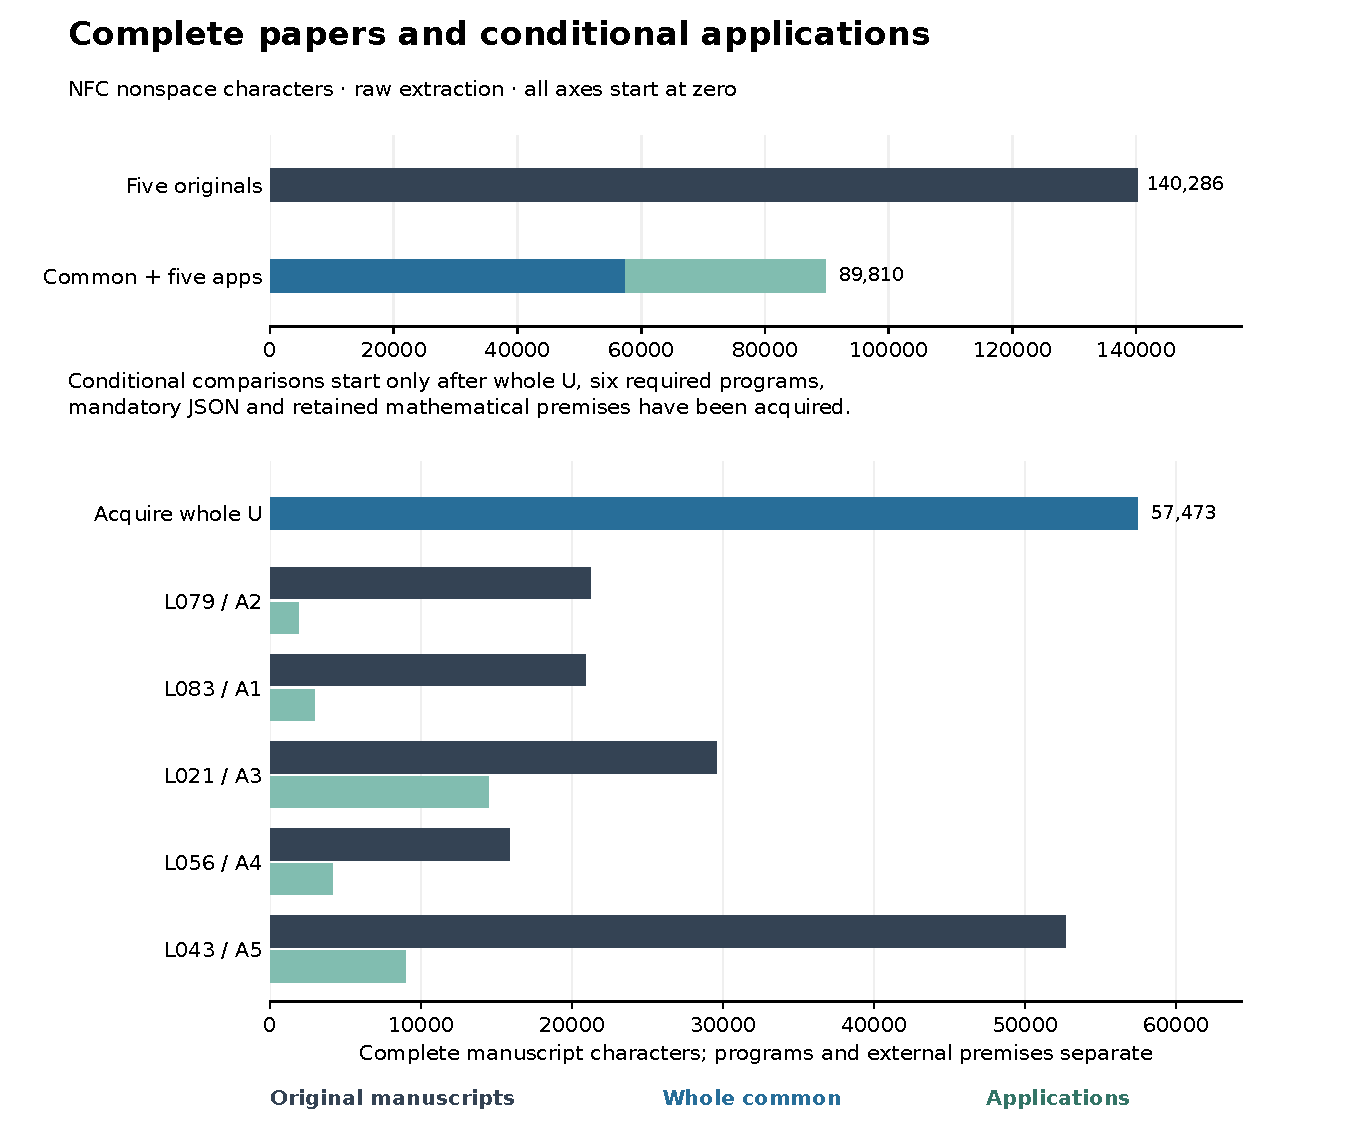
\includegraphics[width=\textwidth]{costs.pdf}\end{center}
The upper graph charges the whole common paper and every application. The lower graph shows the common acquisition cost and all five complete source/application pairs. It is a document-cost picture, not a theorem-dependency graph or a minimality claim. Full required software and external premises are separate; no reduction in their cost is inferred from shorter application bars.

\textbf{Symmetric software boundary.} The five sources and six replacement scientific papers contain no executable listings. Mathematical tables, relations, matrices and algorithm prose remain on both sides. Required and optional replacement programs are outside this manuscript coordinate; their complete inventories are retained. Historical source software costs are unknown, so every software-inclusive factor remains null.
\newpage
\textbf{Complete separate inventories.}
\begin{center}\begin{tabular}{lrrr}\toprule
Whole files & Count & NFC nonspace chars & Literal bytes\\\midrule
Required programs & 6 & 22,870 & 27,832\\
Mandatory JSON & 1 & 1,602 & 3,982\\
Optional validation & 6 & 13,633 & 15,153\\
Operational drivers & 5 & 28,351 & 30,900\\
Partial Lean files & 7 & 24,437 & 33,350\\
\bottomrule\end{tabular}\end{center}
The 20-page required appendix contains 24,904 primary characters and includes the complete mandatory JSON. The seven-page optional appendix contains 13,974 characters. Printed and raw forms are alternatives, never additive. Required status is unchanged: the six finite-proof programs and certificate data remain prerequisites. The seven Lean files support 42 scoped declarations (nine new), not full source formalization.

For historical accuracy, L043 names \emph{Magma} and the \(L_2\)-quotient algorithm. Three frozen input metadata fields incorrectly say GAP; our implementations use GAP and Python. This explicit attribution correction changes neither counts nor program roles.

\textbf{Sensitivity of the whole written factor.}
\begin{center}\small\begin{tabular}{lrrr}\toprule
Unit & Raw & Selected & Calibrated\\\midrule
NFC: Whitespace tokens & 1.745387 & 1.733929 & 1.733929\\
NFC: Alphanumeric units & 1.788109 & 1.774932 & 1.774932\\
NFC: Nonspace characters & 1.562031 & 1.544990 & 1.544990\\
NFC: Collapsed-space characters & 1.595095 & 1.579025 & 1.579025\\
NFC: Collapsed UTF-8 bytes & 1.499777 & 1.484640 & 1.490172\\
NFKC: Whitespace tokens & 1.748277 & 1.736823 & 1.736823\\
NFKC: Alphanumeric units & 1.788109 & 1.774932 & 1.774932\\
NFKC: Nonspace characters & 1.564729 & 1.547694 & 1.547694\\
NFKC: Collapsed-space characters & 1.597820 & 1.581755 & 1.581755\\
NFKC: Collapsed UTF-8 bytes & 1.626911 & 1.610559 & 1.610559\\
\bottomrule\end{tabular}\end{center}
``Selected'' removes only the exact accepted running furniture. ``Calibrated'' additionally uses the accepted event-bound glyph repairs; brace pieces and mapsto strokes are disclosed text proxies, not reconstructed layout. Both normalizations and all five units are retained: 30 coordinates and 180 exact fractions are supplied in JSON and CSV. The primary coordinate was fixed before evaluation; it was not chosen from these factors.

Full graphical and formula-layout costs, classical external proofs, historical software, catalogue construction and complete formalization costs remain unknown, not zero. Retained inputs include Dickson/Giudici subgroup results, projective automorphisms, Schulte--Weiss and McMullen--Schulte geometry, the character estimate, finite-field facts, and the Dirichlet/Suzuki inputs to L021. Full costs are not silently supplied by another topic. The exact accepted input and scientific review manifests are bound in the portable packet; this numerical author also authored the expanded science. A distinct arithmetic review is still required.
\end{document}
